\section{Introduction} \label{introduction}
T cells are a crucial component of a well-regulated immune system. The large variability in the T-cell receptor (TCR) sequence enables TCRs to recognize a diverse selection of pathogens. This thesis will describe approaches to improve predictions and the understanding of TCR specificity. This will allow for a better understanding of the immunogenicity of antigens and further the research within vaccine development and cancer.

\subsection{The Immune System}
Here, an introduction to the core aspects of the immune system is given, which serves as this project's foundation. The primary source for this section is \textit{Janeways Immunobiology} \cite{Murphy2008JanewaysImmunobiology}.

The immune system consists of various mechanisms to recognize and combat pathogens, cancer cells or parasites. The immune system generally consists of the fast and unspecific innate immune system, which recognizes a variety of conserved pathogen-associated molecular patterns \cite{Gasteiger2017CellularPlayers}. The innate immune system is present from birth and acts as our first line of defence against pathogens that have penetrated the skin or other external barriers. The adaptive immune system generates a slow and specific response to pathogens, which can recognize virtually any antigen a pathogen expresses. The immunity gained from this system is learned through the organism's lifetime, as it accumulates memory of previous infections. The primary cell types involved in the adaptive immune response are lymphocytes. Lymphocytes primarily consist of T-cells and B-cells, expressing immunoglobulin receptors to recognize foreign pathogens. A vital component of the adaptive immune system is the ability to remember signals from past infections and initiate a swift and robust immune response in case of subsequent infections. This ability is gained by having long-lived memory T and B-cells, which can be activated and undergo clonal expansion to quickly generate enough cells to combat the infection \cite{Murphy2008JanewaysImmunobiology}. 

During development, T-cells either become CD4+ helper T-cells or CD8+ effector cells. This project will focus on the CD8+ effector T-cells and their recognition of peptides displayed in Major histocompatibility complex (MHC) class I molecules. These T-cells are responsible for killing infected cells by initiating apoptosis to stop a current infection. While CD8+ T-cells are essential for combating intracellular pathogens, many additional steps are required for a successful immune response, such as the recruitment of CD4+ helper T-cells \cite{Chaplin2010OverviewResponse}.

%Fokus kun på MHC class I og de cellulære response. Men forhåbenligt kan det scales til begge classes når data bliver abundant nok.
\subsubsection{MHC class I Displays Antigens to CD8+ T cells}
Almost all cells in the human organism contain MHC-I. The MHC-I sit embedded in the cell membrane, allowing cells to show their intracellular contents to CD8+ T-cells.

Proteins inside a cell are continuously monitored for foreign proteins (Figure \ref{fig:mhc_presentation}). A protein is fragmented into smaller peptide fragments. These fragments are then moved into the endoplasmic reticulum through the transporter associated with antigen processing (TAP), where they are incorporated into an assembled MHC-I \cite{Abele2004TheProcessing}. After the pMHC complex is formed, the pMHC is transported to the cell surface through a vesicle. From here, the T-cells can assess the presence of non-self peptides bound on the cell surface in complex with MHC-I.

\begin{figure}
    \centering
    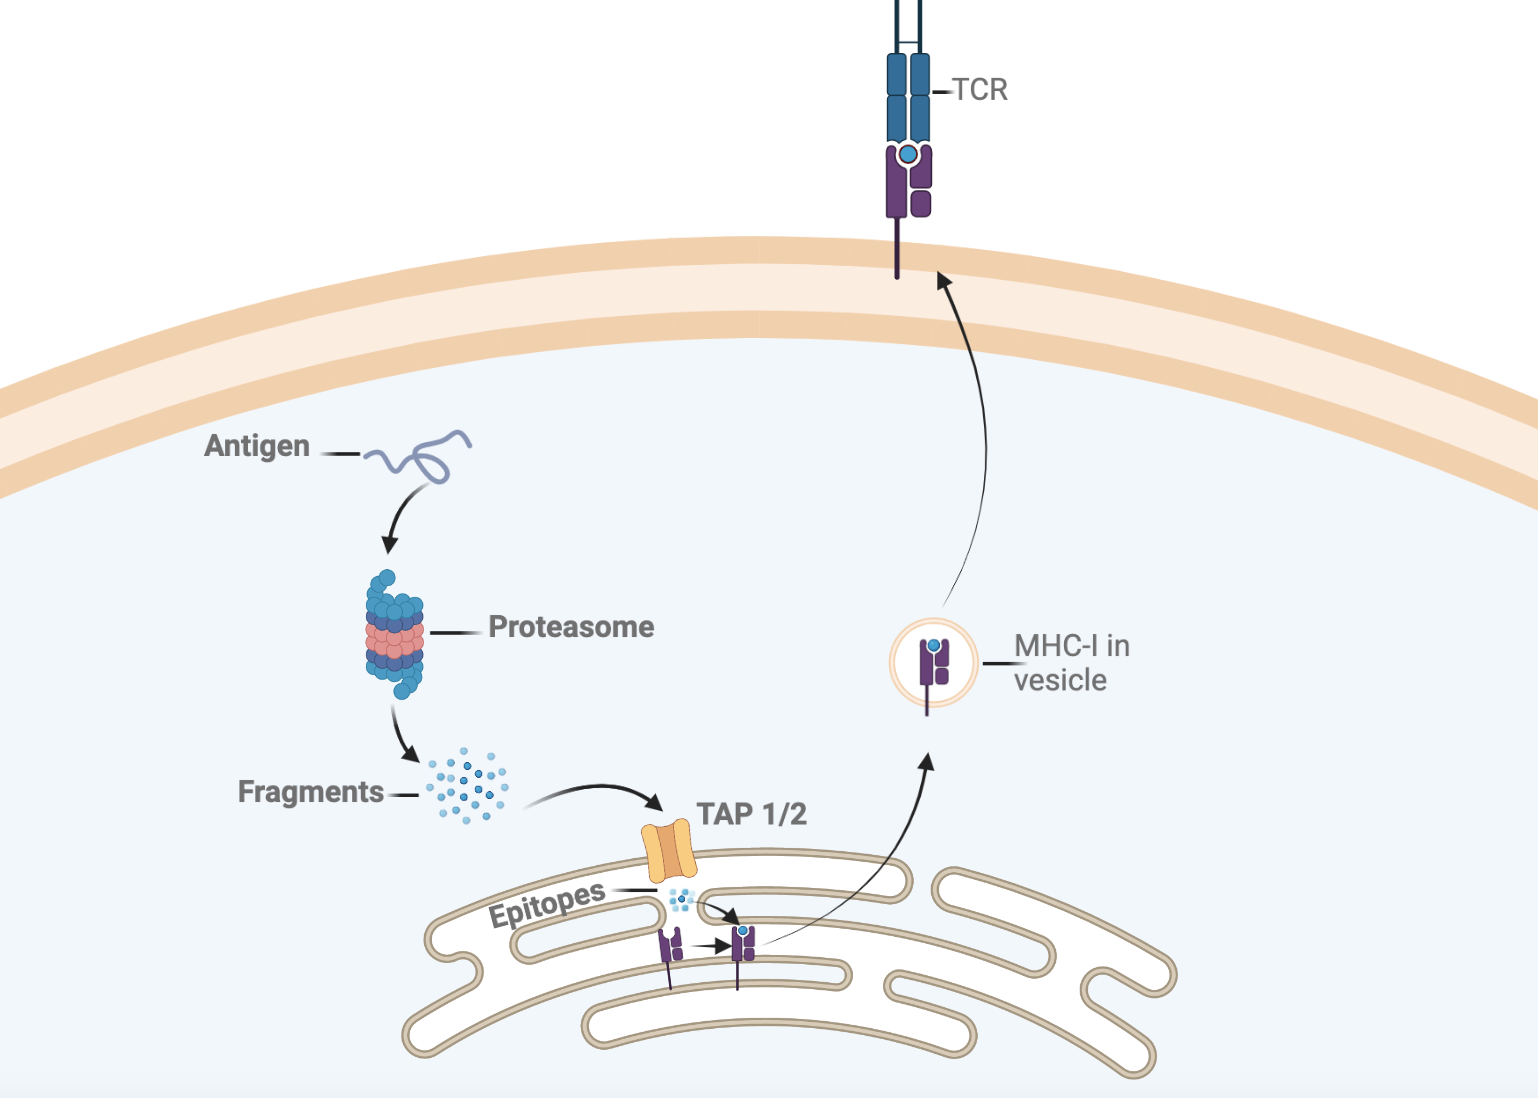
\includegraphics[width=\linewidth]{figures/MHC_representation.png}
    \caption{Infected cell displays epitopes to T-cells by incorporating the epitopes into an MHC class I molecule. The newly created pMHC molecule is transported to the surface and displayed to roaming CD8+ TCRs.}
    \label{fig:mhc_presentation}
\end{figure}

% Creation af TCR
\subsubsection{TCRs interacts with Antigen using hypervariable regions}
The adaptive immune system needs to recognize a large number of pathogens to protect the body. The molecule responsible for recognizing diverse foreign peptides from pathogens are TCRs. TCRs need to recognize peptides from virtually any pathogen, which poses the issue of generating a molecule with enough diversity to recognize any peptide.

T-cells uses gene rearrangement to generate diverse TCRs \cite{Krogsgaard2005HowAntigen, Davis1988T-cellRecognition}. A TCR is a complex of two subunits (TCR{\textalpha} and TCR{\textbeta}) connected by a disulfide bond. Each subunit consists of a variable and constant domain. The variable domain is responsible for interactions with epitopes displayed on pMHC molecules and is created through gene rearrangement (Figure \ref{fig:tcr_generation}). The TCR{\textalpha} is generated by randomly joining a V and J segment, while the TCR{\textbeta} is created by joining a V, D and J segment. Many V, (D), and J gene segments are available at the TCR{\textalpha} and TCR{\textbeta} loci, and the possible combinations of V, (D) and J gene segments generates a large portion of the T-cells' diversity. Additional diversity is introduced by adding random nucleotides in the junctions between the V, (D) and J segments. These nucleotides result in random amino acids at the junctions between the V, (D) and J gene segments. The fact that TCR{\textalpha}s and TCR{\textbeta}s are generated separately gives additional diversity, as any two TCR subunits could have been generated and combined to a full TCR. The introduced diversity means that it is possible to generate upwards of $10^{18}$ possible unique TCRs. However, while the number of possible TCRs is quite large, the number of possible epitopes that T-cells need to recognize is much larger than the number of T cells present at any one time. Therefore, while T-cells are rather specific towards certain peptides, they need to be able to recognize multiple peptides \cite{Sewell2012WhyCross-reactive, Glanville2017IdentifyingRepertoire}.

\begin{figure}
    \centering
    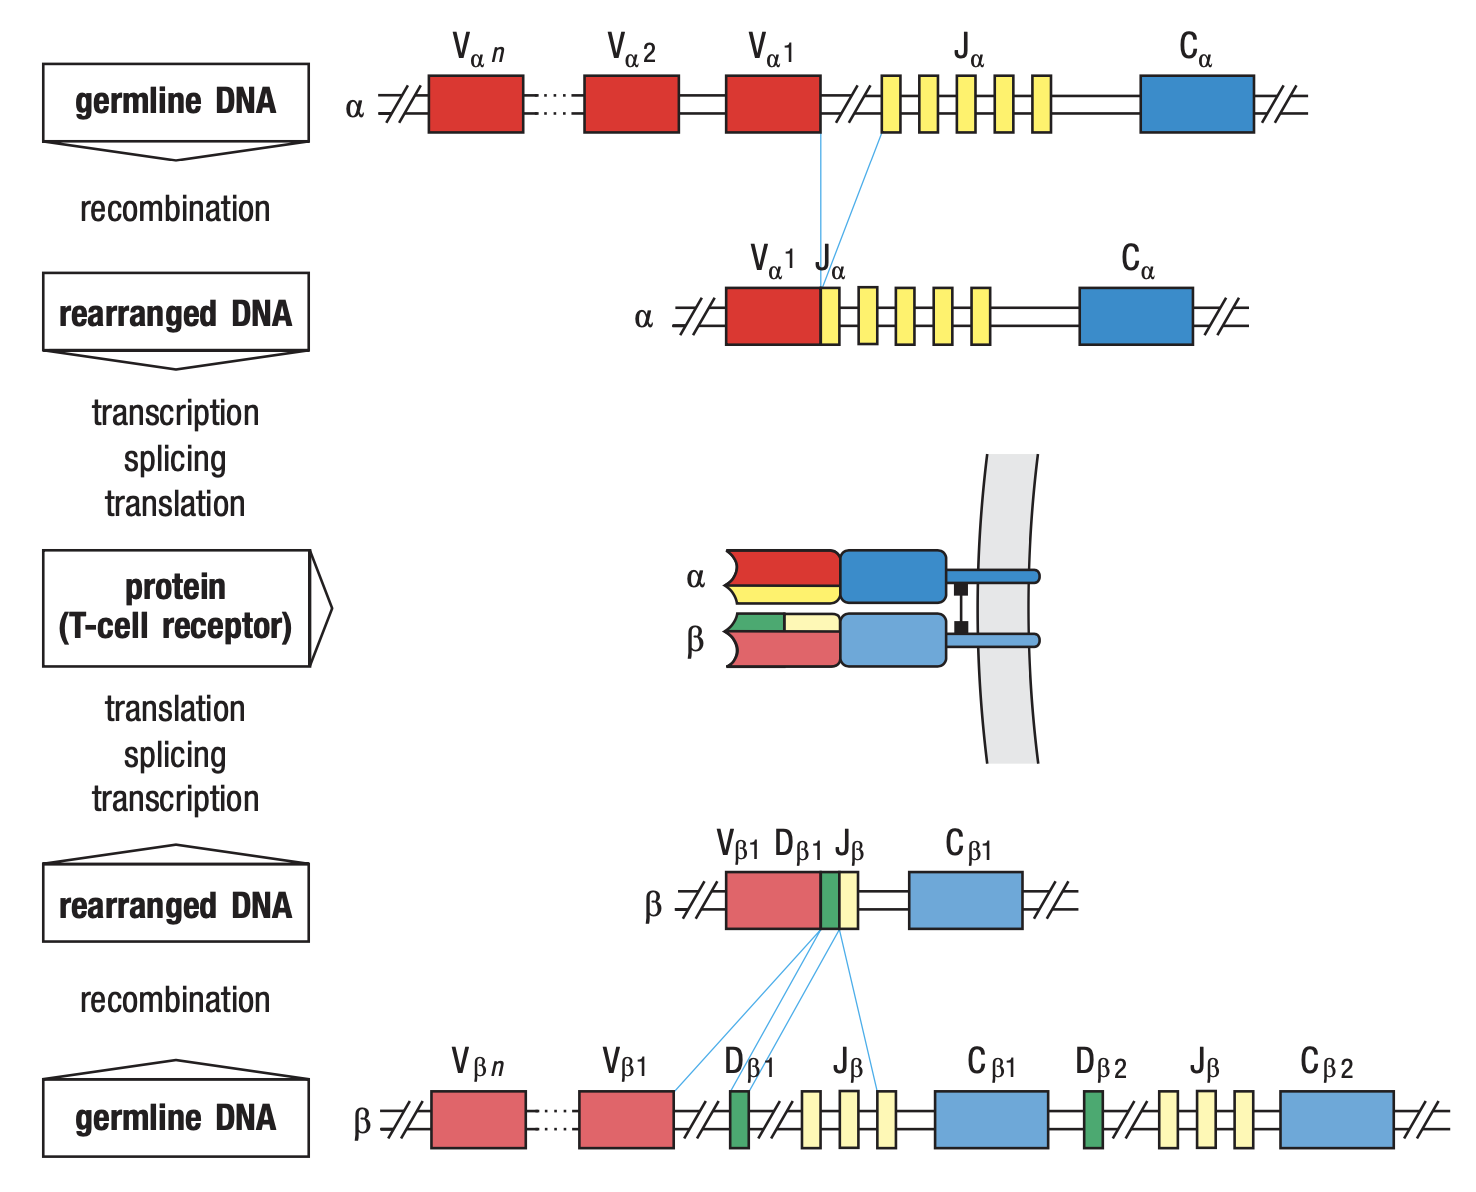
\includegraphics[width=0.8\linewidth]{figures/tcr_generation.png}
    \caption{The DNA sequences for TCRs are generated through gene rearrangements of both the {\textalpha} and {\textbeta} locus. A V, (D for the {\textbeta}) and J segment are randomly selected and generate the variable domain of the TCR. Figure adapted from \cite{Murphy2008JanewaysImmunobiology}.}
    \label{fig:tcr_generation}
\end{figure}

The variable domain of the TCR is made up of an immunoglobulin fold. This fold contains two beta-sheets folded onto each other in a {\textbeta}-sandwich structure \cite{Bork1994TheCore}. The {\textbeta}-sheets consist of conserved amino acids, while the loops connecting the sheets are less conserved and contain most of the diversity in the TCR. Each of the two TCR subunits contains three of these loops, which are collectively referred to as Complementarity-Determining regions (CDRs). These CDRs are essential for epitope binding and are the structures closest to the actual peptides (Figure \ref{fig:tcr_xray}). CDR1 and CDR2 are encoded directly in the V gene, while  CDR3 consists of both the V, (D) and J segments and nucleotides introduced at the junctions. The CDR3s, therefore, have a higher level of diversity than the other CDRs and are also thought to be the most important for epitope binding \cite{Tsuchiya2016TheLoops}. Especially the CDR3b has been widely investigated, as the D gene segment allows for much diversity at the CDR3b \cite{Rossjohn2015TMolecules}. Furthermore, the CDR3s are generally in closer contact with the peptide than CDR1 and CDR2, which also interacts with the MHC molecule (Figure \ref{fig:tcr_xray}).
% immunoglobulin fold og hvordan det skaber CDRs
\begin{figure}
    \centering
    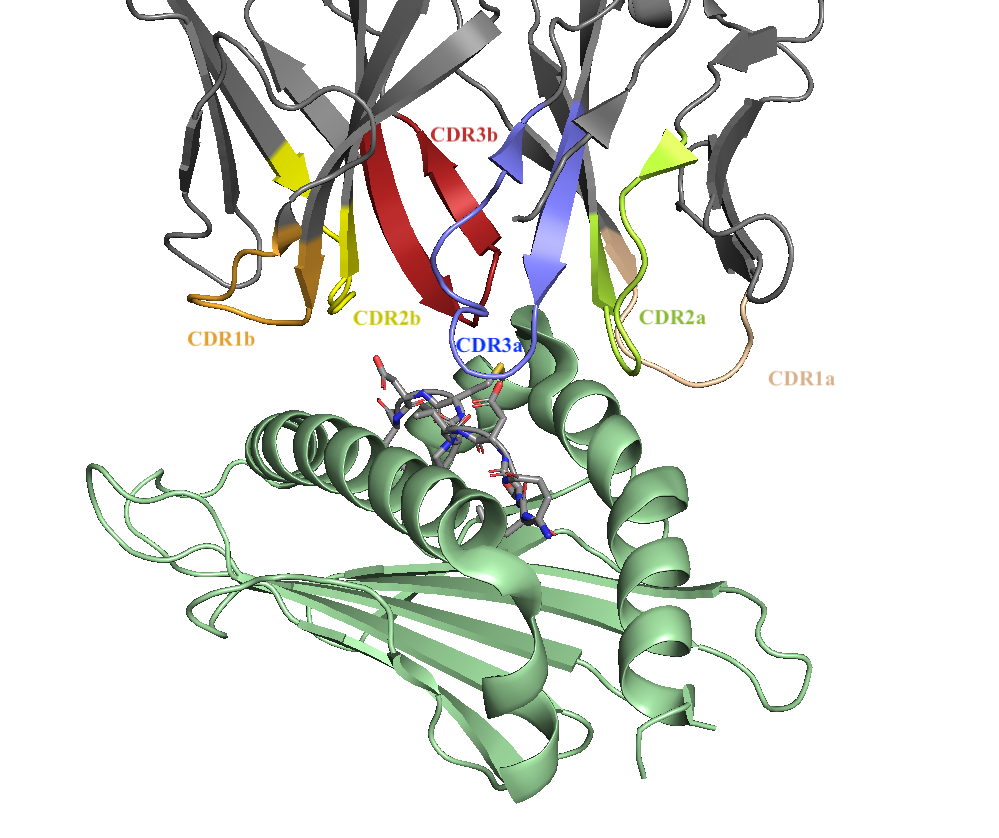
\includegraphics[width=0.65\linewidth]{figures/tcr_pmhc_xray.png}
    \caption{The TCR (top) interact with the pMHC (bottom) complex predominately through the CDR loops at the end of the TCR. Visualization created in PyMOL \cite{SchrodingerLLC2015The1.8} using PDB structure 3TFK \cite{Adams2011TComplex}}
    \label{fig:tcr_xray}
\end{figure}

\subsection{Machine Learning Methods}
Predicting TCR-pMHC interaction is a supervised classification problem. In these types of problems, a model is fitted to predict the most likely class for a given observation.
$$ y = f_{\theta}(\textbf{X})$$
The model $f_{\theta}$ is parameterized by weights $\theta$ and takes the input \textbf{X} and attempts to predict the output class y. Predicting TCR-pMHC binding is a binary classification meaning $y=1$ refers to binding while $y=0$ refers to non-binding.

Deep learning is a sub-field of machine learning utilizing artificial neural networks for statistical modelling. These types of networks mimic the brain in the way neurons signal and activate each other in specific patterns to generate a specific output. The simplest type of artificial neural network is the feedforward neural network (FFN). Figure \ref{fig:feed_forward} depicts a FFN with one input, hidden and output layer, each containing several neurons. Creating predictions with a neural network is called a forward pass. Here, the output of a layer is calculated from the previous layer, which is repeated for all layers. The output of a neuron is calculated from the previous layer by taking a weighted average of the outputs of the previous layers. This average is then passed through a non-linearity to generate the output of that given neuron.

The learnable parameters in a FFN are the weights used to generate the weighted averages. When the model has generated predictions through the forward pass, these weights can be updated through a method called backpropagation. A loss function such as cross entropy or mean square error is used to calculate the loss of the model. The loss gradient is calculated for each weight by backpropagating the gradient through all hidden layers. The weights are then updated using an optimization method such as gradient descent, thereby lowering the training loss. The cycle of predicting observations in the forward pass and propagating the loss gradient backwards is repeated, and weights are updated each iteration until a specified number of epochs has been reached. The extensions of the FFN introduced in the next sections are more advanced in architecture, but all rely on backpropagation to update their weights.

\begin{figure}
    \centering
    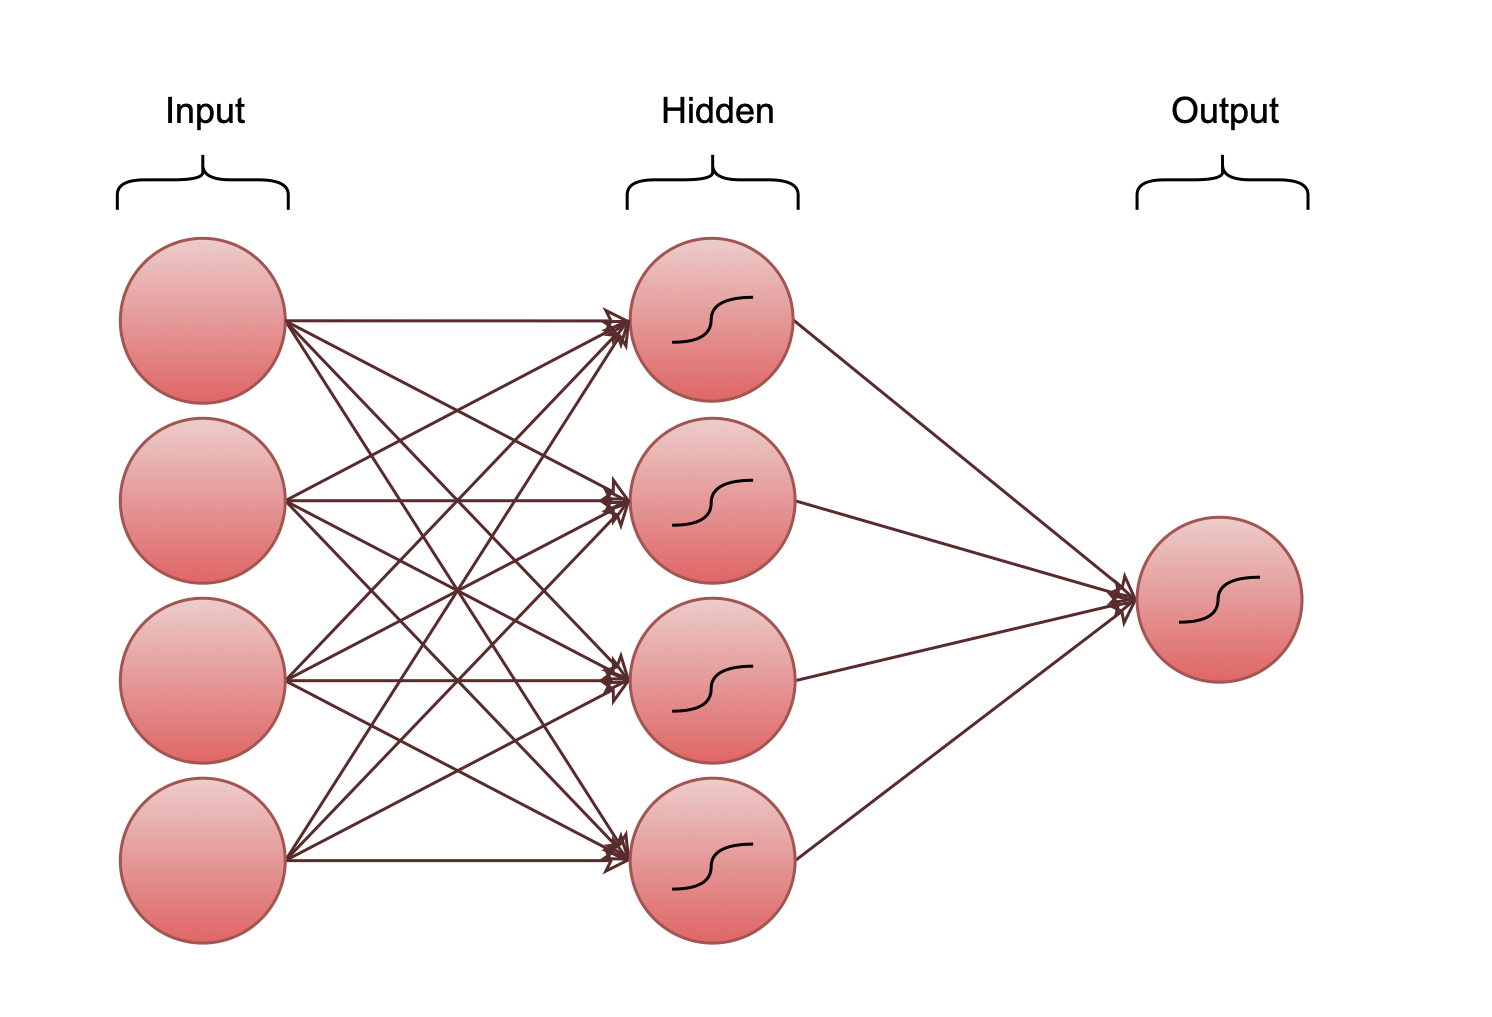
\includegraphics[width=0.75\linewidth]{figures/feed_forward.png}
    \caption{A feedforward network consisting of an input, hidden and output layer. Each circle represents a neuron, and the arrows represent the weights applied when propagating the signal from the previous layer. A non-linear activation function is applied on hidden and output neurons represented by the sigmoid curve.}
    \label{fig:feed_forward}
\end{figure}

\subsubsection{Convolutional Neural Networks} \label{cnn}
FFNs cannot handle sequential data gracefully, as they are highly dependent on data having the same input size. Convolutional Neural Networks (CNNs) handles this by finding local motifs in the input independently of their position. CNNs were initially developed for image analysis to identify certain pixel arrangements, which can then be combined into more complex features resembling e.g. facial features being combined into a face \cite{NIPS2012_c399862d}. CNNs convolute an image by scanning with a filter/kernel with specific weights. These filters obtain a high value in areas where the input matches the weights, generating a feature map specific for that filter. After convolution, the output is transformed using a  non-linear transformation such as hyperbolic tangent (Tanh) function. The feature map's dimensionality can be reduced by max pooling. This operation pools the image by selecting the largest positive value within an area to reduce the image's dimensions and regularize the network.

CNNs have also proven helpful for finding motifs in biological sequences \cite{Jurtz2017AnSolutions, Aoki2018ConvolutionalSequences}. Each filter represents a position weight matrix with a specific motif depending on the weights (Figure \ref{fig:cnn}). The filter scans over the sequence and yields a high output if the sequence resembles the motif stored in the filter (Figure \ref{fig:cnn}). Multiple convolutional and max pool layers can be used to generate a more complex convolution of the sequence. However, for this project, we only investigate shallow one-layer convolutions with a subsequent global max pool, as this type of network has shown promise for modelling TCR-pMHC interactions \cite{Montemurro2021NetTCR-2.0Data}. The resulting feature vector is made by having multiple filters scan the sequence and represents whether the motifs encoded by the filters were present in the sequence. Downstream modelling then decides whether the presence of these motifs result in an interaction or not.
% desribe how the CNN scans the sequence and generates an activation value, and how that is then selected by maxpooling

\begin{figure}
    \centering
    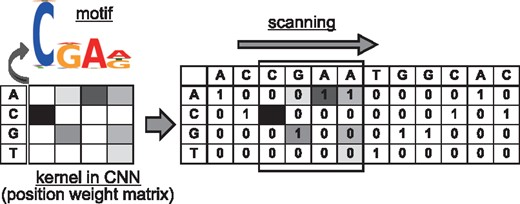
\includegraphics[width=0.9\linewidth]{figures/cnn.jpeg}
    \caption{A kernel/filter scans the entire sequence looking for a similar motif. The filter finds a complete match (marked by a box). The subsequent max pooling operation will then select this match. Figure adapted from \cite{Aoki2018ConvolutionalSequences}}
    \label{fig:cnn}
\end{figure}

\subsubsection{Long Short Term Memory}
Recurrent neural networks (RNN) can also model sequential data. These networks propagate the signal through the sequence by using the previous state in the calculations. The simplest RNN can be challenging to train as the loss gradient starts to vanish when the hidden states are propagated through the sequence. When the gradient vanishes, it becomes hard for the network to update weights, as a gradient is required for updating the weights. Long short-term memory (LSTM) was introduced to solve this issue by allowing the signal to bypass most of the matrix multiplication and thereby alleviate the problem with vanishing gradients \cite{hochreiter1997long}.

An LSTM consists of an LSTM cell for each input in the sequence (Figure \ref{fig:lstm}). The input for a given cell is the input at that position ($x_i$), the previous cell state ($c_{i-1}$), and the previous hidden state ($h_{i-1}$). The cell state represents the long-term memory of the LSTM used to avoid the vanishing gradient, whereas the hidden state is the working memory and also serves as the model's output. Four gates exist in the LSTM, each consisting of a dense layer and an activation function (yellow blocks in Figure \ref{fig:lstm}). The forget gate ($f_t$) calculates how much should be forgotten of the current cell state (c) by a sigmoid layer, followed by elementwise multiplication. The input gate (i) determines how much new information should be integrated into the cell state, while the next gate (\v{c}) determines what should be integrated. Lastly, the output gate (o) calculates the new hidden state, fed to the next cell along with the updated cell state.

There exists two common methods for using LSTMs depending on the problem at hand. Using the hidden state for each cell can often be beneficial in a many-to-many problem such as amino acid structure prediction, as we want information about each individual residue. At the same time, many-to-one problems, such as predicting TCR-pMHC interactions, often uses the last hidden state in the sequence. At this state, information from all previous positions has been incorporated into the model, allowing the model to condense information about all positions into one hidden state.

\begin{figure}
    \centering
    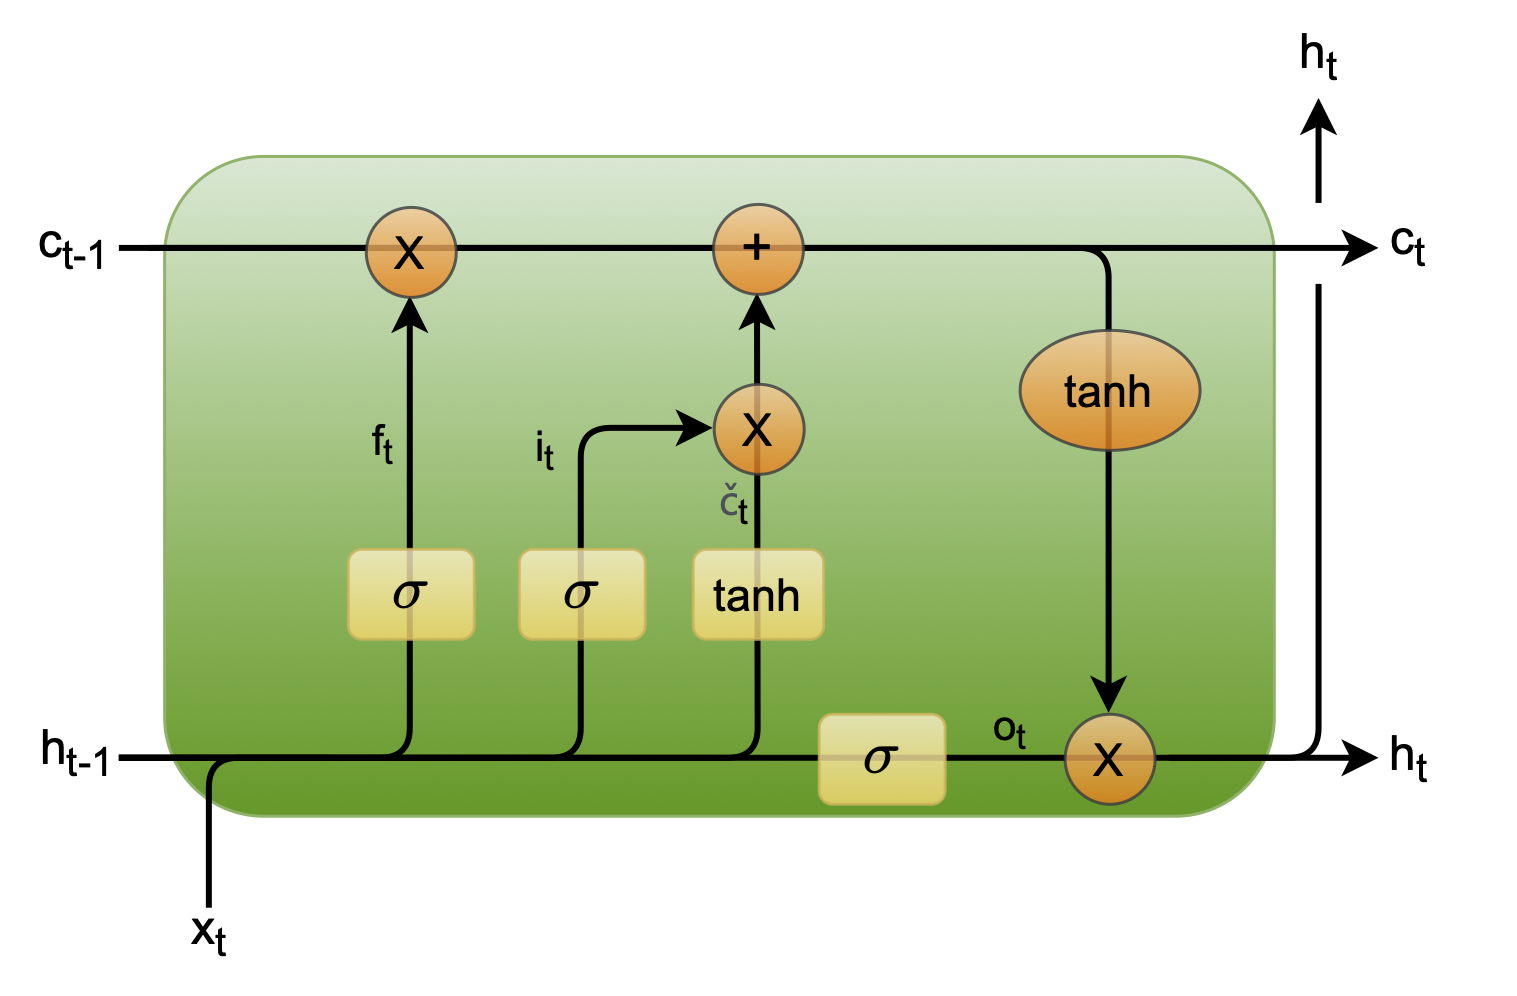
\includegraphics[width=0.9\linewidth]{figures/lstm.png}
    \caption{Visualization of operations and layers present in an LSTM cell. The previous hidden state and the new input is concatenated. Each gate determines what should be forgotten (f), how much should be added (i) and what should be added (\v{c}) to the cell state. The last gate determines how to combine the new input, hidden state and cell state in the output.}
    \label{fig:lstm}
\end{figure}

\subsubsection{Attention Mechanism} \label{section:attention}
While the last hidden state in LSTMs incorporates information from all states in the sequence, information may still be lost, especially if the first positions of the sequence are important. Instead, attention can be used to focus on important areas of the sequence while excluding unimportant areas. By using attention, the hidden state for each position can be incorporated into an overall hidden state, which means all states can be used instead of only using the final hidden state even for a many-to-one problems such as TCR-pMHC binding.

Attention mechanisms were first developed for machine translation, where words placed in certain areas would contribute more to the prediction of words in the translated text \cite{Bahdanau2014NeuralTranslate}. Another widespread use of attention is transformers, which uses self-attention to understand languages \cite{Vaswani2017AttentionNeed, Devlin2019BERT:Understanding}.

Within biological sequence analysis, attention has been used for predictions of subcellular location of proteins \cite{AlmagroArmenteros2017DeepLoc:Learning}, where the signal peptide stores hold most of the information about its subcellular location. Similarly, the CDRs contain most of the information from TCRs, which can be selected using attention.

In order to calculate the attention on a position, all hidden states from the LSTM output are used $(h_1, h_2 ... h_L)$, where L represents the sequence length. The attention function (Equation \ref{eq:att}) is used to calculate the similarity of each hidden state to a high-level query vector (\textbf{q}) and then scaled using the softmax function (Equation \ref{eq:softmax}). Here the query vector (\textbf{q}) and the weight matrix ($\boldsymbol{W_k}$) are learnable parameters learned during training.
\begin{equation}
    e_l = Tanh(\boldsymbol{h_l}\boldsymbol{W_k})\boldsymbol{q}^T
    \label{eq:att}
\end{equation}
\begin{equation}
    a_l = \frac{\exp{e_l}}{\sum_{i=1}^L\exp{e_i}}
    \label{eq:softmax}
\end{equation}
Lastly, a hidden state can be calculated with the context of all hidden states.
\begin{equation}
    \boldsymbol{h_c} = \sum_{l=1}^L a_l\boldsymbol{h_l}
\end{equation}

A schematic version of these calculations, along with the dimensions of the vectors, can be seen in Figure \ref{fig:attention_schema}. The attentions for each position can be calculated simultaneously using matrix multiplication to speed up the computations.

The query vector represents how an important hidden state would look. If a hidden state has a vector representation similar to the query vector, their dot product will be large, resulting in a considerable attention value for that position. 
An average of the hidden states weighted by importance can be calculated by first calculating the attention put on each position and then incorporating each hidden state according to this value.


% context vector (q) is a representation of an important residue
\begin{figure}
    \centering
    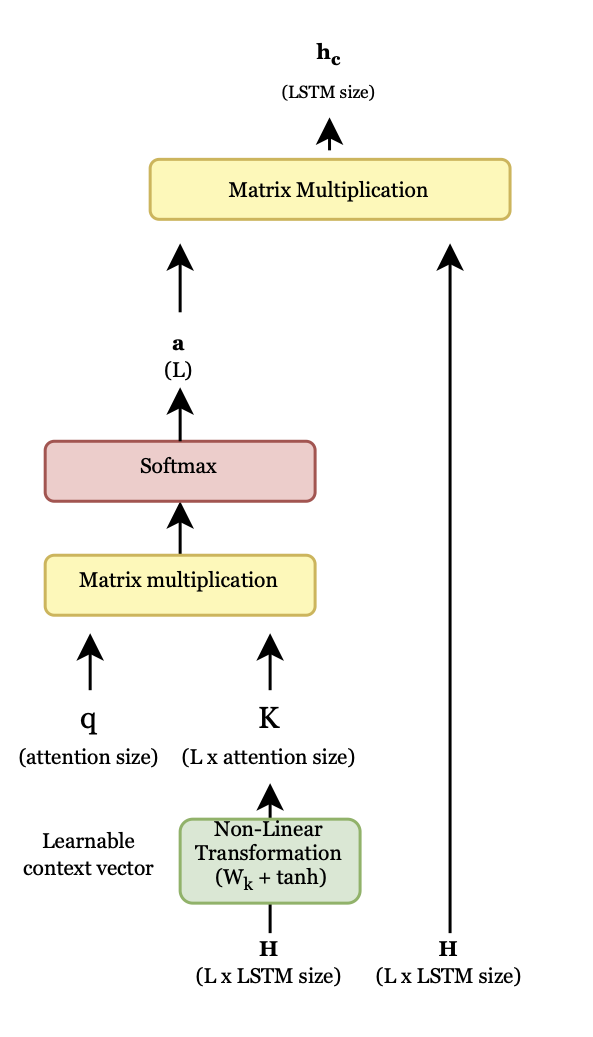
\includegraphics[scale=0.38]{figures/attention_diagram.png}
    \caption{Attention mechanism used for this project. Q (query) is a vector of learnable parameters. K (Key) is created by a linear layer and the Tanh activation function. The matrix-vector product between q and K is scaled using a softmax, and the resulting attention values are then used to create a weighted average using matrix multiplication. Dimensions of matrices and vectors are shown in parenthesis.}
    \label{fig:attention_schema}
\end{figure}

\subsection{TCR-pMHC binding studies can improve vaccine technologies} \label{studies}
The field of immunoinformatics investigates immunogenicity in silico. Knowledge of peptide immunogenicity is essential for designing better vaccines, as peptide-based vaccines allow for better targeting of immunodominant peptides. Also, peptide vaccines are easier to produce because of the simplified construct and could potentially be tailored for specific populations \cite{Kazi2018CurrentDesign}. In contrast, current vaccines often use entire antigens, which may result in a less effective immune response than a peptide-based vaccine with carefully selected peptides \cite{Patronov2013T-cellImmunoinformatics}. 

Peptide-based vaccines both have prospects within cancer therapy and treating various infectious diseases by enhancing the organism's immune system \cite{DeLuca2007TheImmunotherapy}. Knowing the rules for TCR binding will therefore provide a substantial step toward more personalized treatments for vaccinations and cancer treatments.

Predictions tools for immunogenicity by predicting pan-specific pMHC binding, such as NetMHCpan \cite{Hoof2009NetMHCpanHumans,Reynisson2021NetMHCpan-4.1Data}, have existed for a while. However, the immunogenicity of a peptide also depends on additional factors, including TCR binding and stimulation by cytokines \cite{Murphy2008JanewaysImmunobiology}. Multiple tools have also been developed for predicting TCR-pMHC predictions previously \cite{Montemurro2021NetTCR-2.0Data, Chronister2021TCRMatch:Receptors, Springer2020PredictionPairs, IsabellJurtz2018NetTCR:Networks, Wu2021TCR-BERT:Analyses}. These tools use various methodologies from alignment \cite{Chronister2021TCRMatch:Receptors}, to CNN based approaches \cite{IsabellJurtz2018NetTCR:Networks, Montemurro2021NetTCR-2.0Data} and NLP based models using LSTMs \cite{Springer2020PredictionPairs} or transformers \cite{Wu2021TCR-BERT:Analyses} to predict TCR peptide interactions.

In the thesis by Meitil \cite{Meitil2021UsingPrediction} additional force field energy terms were estimated. These energies provide structural information about the TCR-pMHC complex and could be used to increase model performance. Furthermore, a benchmark dataset was also created, serving as the primary data source for this project. 

%early stopping citer introduction to deep learning sequences paper

\subsection{Regularization}
When training machine learning models, it is crucial to have a model that can generalize to unseen data. Regularization techniques exist to avoid having the model overfit on the training set. As overfitting occurs, the model generalizes less as it learns the noise within the training set. One regularization technique is early stopping, where training is terminated after a specified number of epochs without improvement on a validation set \cite{Jurtz2017AnSolutions}. As the model is training, it moves down the loss gradient, which improves the training loss. If the model learns noise specific to the training data, the model will continue to improve on the training data but not on the validation data. Therefore, stopping the model when this occurs avoids learning excessive amounts of noise from the training data.

Another regularization approach is dropout \cite{JMLR:v15:srivastava14a}. Neurons are selected with a random probability and have their value set to 0, effectively removing that neuron from the parameters for one iteration. Therefore, the model cannot rely on a specific set of neurons during training, meaning the model has to find other combinations of inputs to predict binding. By keeping the network in check and forcing it to learn multiple ways of predicting the label, the network is regularized by preventing overfitting to specific inputs.

The easiest way to generate an independent test set is to never use a specific portion for training and only evaluate upon this data. However, if the amount of data is limited, there could be a risk of the test sample being too small and not able to fully represent the variability of the data. Data should not be present in both the training and testing for a proper estimate of the generalization error. Nested cross-validation can use all data for both training and testing (Figure \ref{fig:cv}) and still manage to generate an unbiased estimate of the generalization error. Nested cross-validation works by first dividing data into several partitions. Then two nested loops go over the partitions, where a test partition is selected in the outer loop, while the inner loop selects a validation set for early stopping. A model is trained on the three remaining partitions and used to predict the test set. A new validation set is then chosen, and a new model is trained on the new training partitions. For 5-fold nested cross-validation, models are trained for all combinations of test and validation sets resulting in 20 models and each observation having four unbiased predictions. The final prediction is calculated as the average of the four predictions. Cross-validation can thereby avoid the issues of evaluating performance on data that have been used for training the model but still use all data for training models.
%Crossvalidation
%Early stopping
%Dropout
\begin{figure}
    \centering
    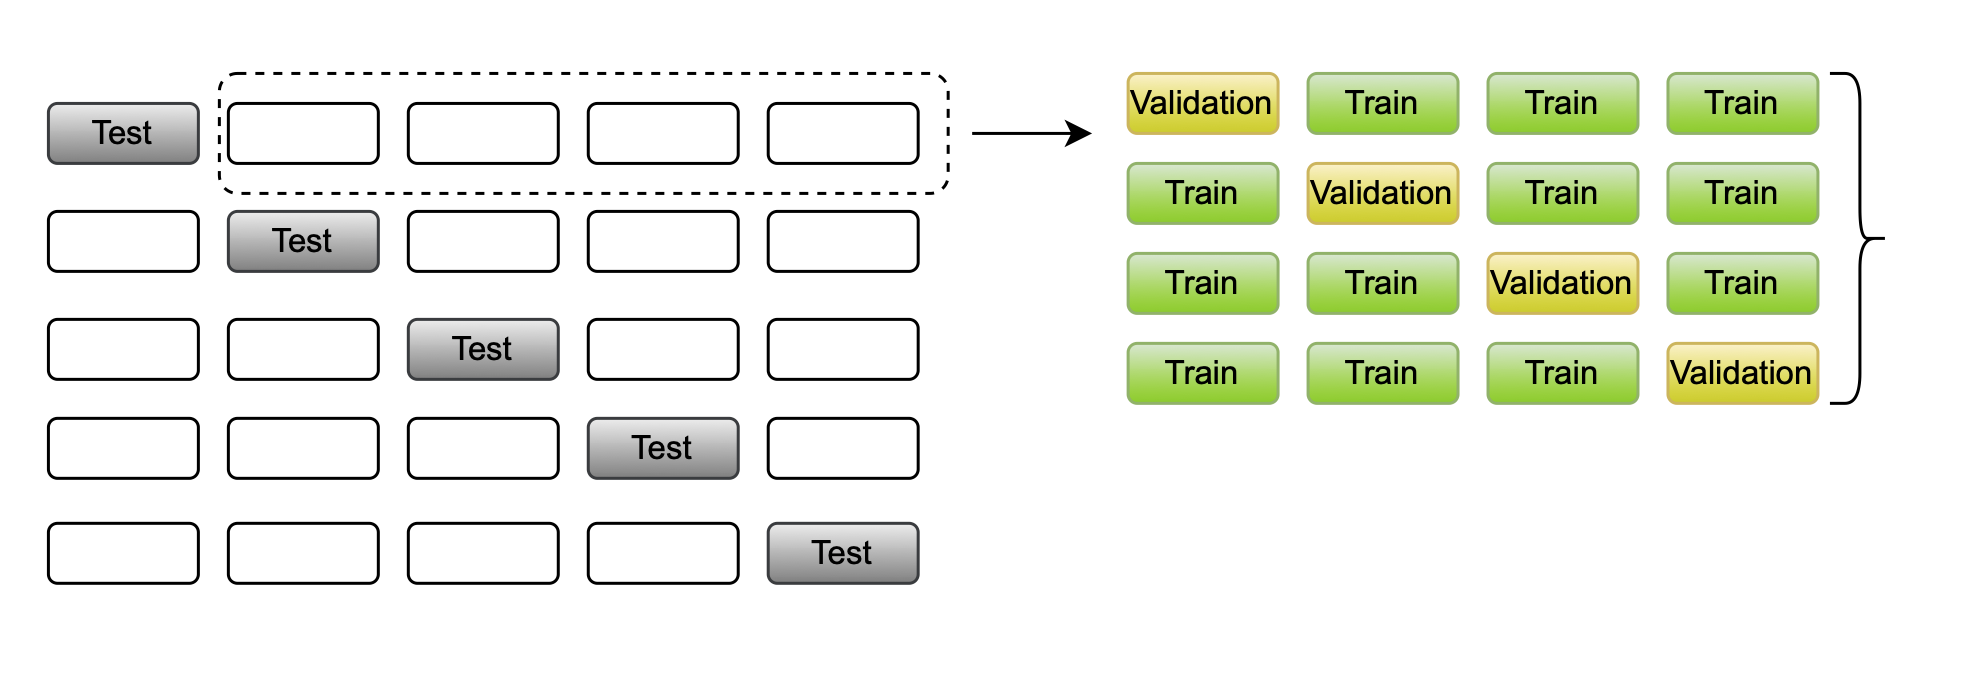
\includegraphics[width=\linewidth]{figures/cross_validation.png}
    \caption{Nested cross-validation to generate test predictions for the entire dataset. The outer cross-validation loop selects a partition for testing, and the inner loop trains for models for each test set, each with a different validation set. After training, 20 models have been trained, and each observation has four predictions. These predictions can then be averaged to generate final predictions.}
    \label{fig:cv}
\end{figure}

\subsection{Methods for Residue Specific Embeddings}
%how skip gram works BLOSSUM
For machine learning, a protein sequence needs to be represented by numerical values. The simplest way to achieve this is by one-hot encoding the sequence. However, representing amino acids as orthogonal vectors does not fully represent the relationship between amino acids. Instead, the sequence can be represented by a Block Substitution Matrix (BLOSUM) encoding \cite{Henikoff1992AminoBlocks}. This encoding captures how some amino acids are closely related and are found more frequently as mutation pairs in nature. When encoding using BLOSUM, amino acids often substituted in nature will be closely related in the encoding space and allow the model to understand how some amino acids have similar functions within proteins.

BLOSUM matrices are generated from homologous proteins and give generic protein-specific encodings representing evolutionary selection. However, CDRs are made by stochastic rearrangement during T-cell development. The BLOSUM encoding may therefore be inappropriate to represent TCR sequences. Within Natural Language Processing (NLP), word embedding methods such as Word2Vec models \cite{Mikolov2013EfficientSpace} are used to learn word embeddings from the context of surrounding words.

These models can be trained using the skip-gram method (Figure \ref{fig:skip_gram}). Here words are used to predict the surrounding words. A selected word is first mapped to a hidden representation (projection) using a single dense layer. This hidden representation is then used to predict surrounding layers using a softmax layer with the vocabulary size as the output dimension. Each ord projection is unique, but the weights used to generate the outputs are shared. Therefore, if words are often found in similar contexts (e.g. king and queen), then the model will give these words similar projections as they are used to predict the same words during training. These projections can then be used in a neural network to embed each word.

When used on proteins, amino acids used in similar contexts would obtain similar embeddings. The Word2Vec model makes it possible to train embeddings specific to CDRs by only including CDR sequences in training. These embeddings may be able to change the input space to be more favourable for predictions of TCR-pMHC interactions.
\begin{figure}
    \centering
    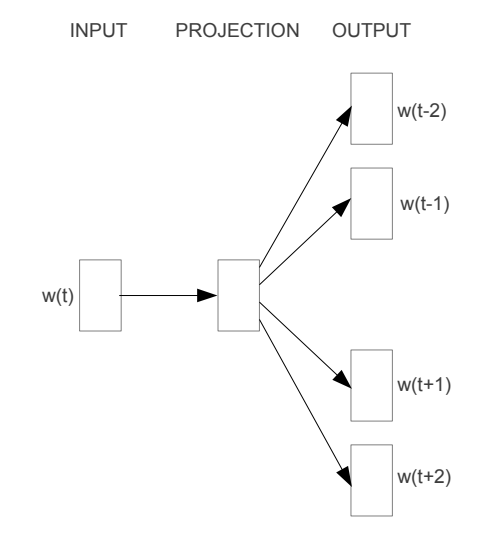
\includegraphics[scale=0.9]{figures/skip_gram.png}
    \caption{The skip-gram algorithm for training Word2Vec models. A word is selected from the input and projected using a linear layer. This projection is then used to predict output words \cite{Mikolov2013EfficientSpace}.}
    \label{fig:skip_gram}
\end{figure}

\subsection{Performance measures}
%AUC
The performance of a model can be measured by many different measures. In binary classification, a confusion matrix is an excellent way of visualising the errors a model makes (Figure \ref{fig:performance_measures}A). The confusion matrix is based on the True Positives (TP), False Positives (FP), False Negatives (FN) and True Negatives (TN) from comparing predictions with their actual class. These classifications can be used in various metrics to evaluate performance.

The most straightforward quantitative performance metric is accuracy, which measures the fraction of correctly predicted observations.
\begin{equation}
    Accuracy = \frac{TP+TN}{TP+FP+FN+TN}
\end{equation}
However, accuracy is ill-suited for unbalanced data, as an accuracy above random (0.5) is easily achievable by only predicting the dominant class. Instead, the area under the receiver operator characteristic curve (AUROC) or simply the area under the curve (AUC) is used. The receiver operator characteristic (ROC) curve consists of the true positive rate (TPR) and false positive rate (FPR).
\begin{equation}
    TPR = \frac{TP}{FP+TP}
\end{equation}
\begin{equation}
    FPR = \frac{FP}{FP+TP}
\end{equation}

The ROC curve is calculated by varying the threshold required for classifying a positive in the interval $\theta \in (0,1)$ and for each possible threshold, calculate the TPR and FPR (Figure \ref{fig:performance_measures}B). Firstly the threshold is so high that all observations are assigned as negatives. As the threshold is lowered, the TPR and FPR increase as more observations are classified as positives until the ROC curve reaches (1, 1), and all observations are classified as positive. The ROC curve will be roughly linear at random performance and give an AUC of 0.5. If the model manages to separate the positive and negatives perfectly, there will be no overlap in the positive and negative score distributions. Therefore, when varying the threshold, the TPR will become one before the FPR changes from 0, yielding an AUC of 1 at perfect performance. For this project, we will primarily use the AUC as it can handle unbalanced data more gracefully than the accuracy metric while still being easy to interpret.
\begin{figure}
\centering
\begin{subfigure}[b]{0.47\textwidth}
   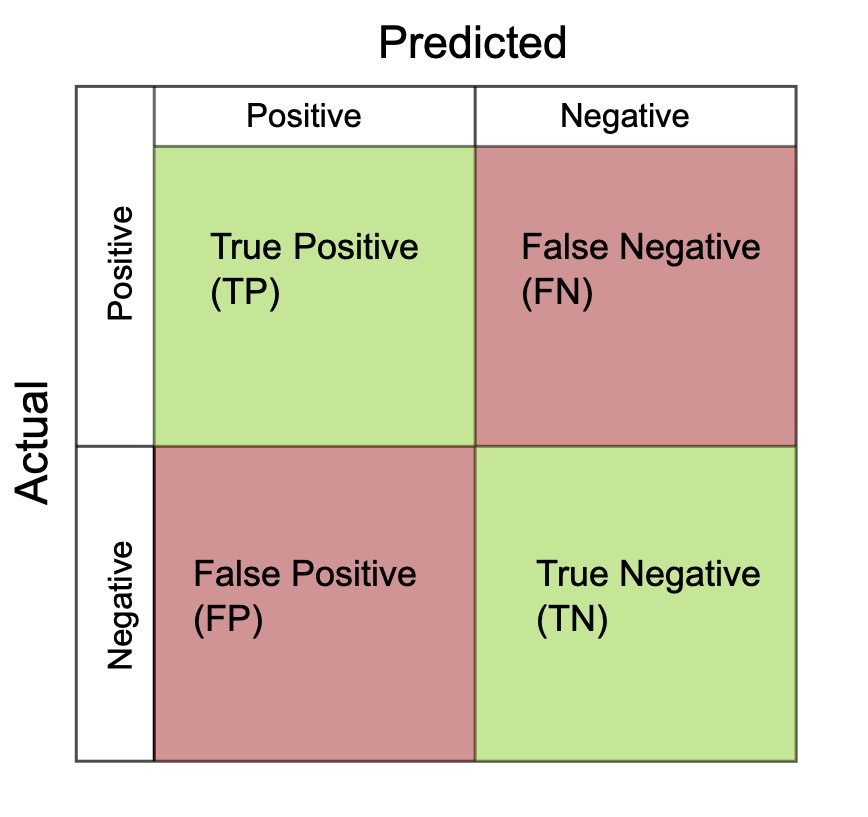
\includegraphics[width=1\linewidth]{figures/confussion_mat.png}
   \caption{}
\end{subfigure}
\begin{subfigure}[b]{0.47\textwidth}
   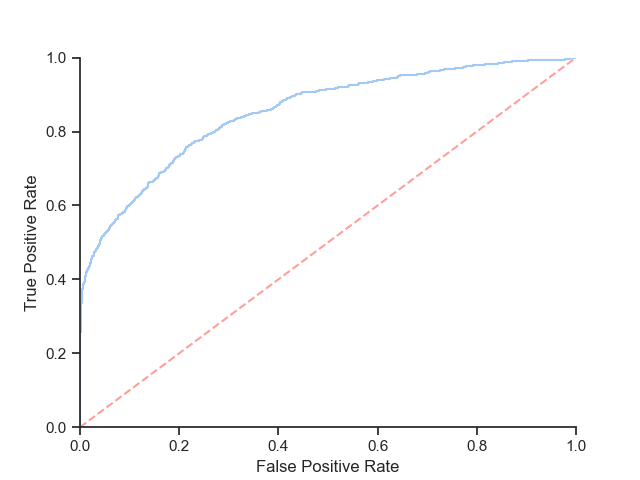
\includegraphics[width=1\linewidth]{figures/ROC_curve.png}
   \caption{}
\end{subfigure}
\caption{\textbf{(A)} Confusion matrix for a binary classifier. \textbf{(B)} Receiver Operator Characteristic (ROC) curve for a binary classifier. Random performance is shown by the dashed red line (AUC = 0.5).}
\label{fig:performance_measures}
\end{figure}


\subsection{Project scope}
The primary goal of this project is to train a classifier to predict TCR-pMHC binding using deep learning and assess its performance. This thesis springs from work done by Meitil \cite{Meitil2021UsingPrediction}, which had a large focus on creating force field energy terms to assist in predicting TCR-pMHC binding. 

In this thesis, the focus will be primarily on using the dataset created in Meitil's thesis. Here we will be evaluating the importance of the sequences and features in the available dataset to see if any sequences or features are irrelevant for TCR-pMHC predictions using a simplified version of the CNN from Montemurro et al. \cite{Montemurro2021NetTCR-2.0Data}. Furthermore, we will introduce a network architecture comprising of Seq-to-LSTM-to-Attention-to-Dense. The model behaviour will be investigated by visualizing the importance of specific positions in the CNN and attention-based LSTM. 

Additionally, the effect of adding attention will be investigated by comparing its performance to models similar to the ones described in Section \ref{studies}. Lastly, the performance gained from having a pan-specific model will be explored by comparing it to two kinds of peptide-specific models.

In this thesis, we want to answer the following questions:

\begin{itemize}
    \item Which sequences and features from the dataset developed by Meitil carry the most information?
    \item Can attention mechanisms be used to distinguish positive and negative CDR3 sequences?
    \item Is the attention mechanism able to preserve performance as data redundancy is reduced?
    \item Can pan-specific models outperform peptide-specific models?
\end{itemize}